\documentclass{beamer}
\mode<presentation> {
\usetheme{Madrid}
\setbeamercovered{transparent}}
\usecolortheme{beaver}
\usepackage[czech]{babel}
\usepackage[utf8]{inputenc}
\usepackage{times}
\usepackage{graphics}
\usepackage{amsmath, amsthm, amssymb}
\usepackage{hyperref}
\title{Malware}
\author{\texorpdfstring{Tomáš Zubrik \ \newline\url{xzubri00@stud.fit.vutbr.cz}}{Author}}
\institute{Vysoké učení technické v~Brně \\Fakulta informačních technológií}
\date{25. 4. 2017}

\addto\captionsczech{\renewcommand{\figurename}{Obrázok}}

\begin{document}
\begin{frame}
\titlepage
\end{frame}
%-------------------------1st page-------------------------
\begin{frame}
\frametitle{Malware}
\begin{itemize}
\item{\textbf{Malware} (skratka z~anglického malicious software) alebo malvér je
všeobecné označenie škodlivého softvéru}
\item{Zaraďujeme tu vírusy, trójske kone, spyware, adware a~mnohé ďaľšie}
\item{Malware sa šíri do užívateľských počítačov zvyčajne prostredníctvom internetu}

\begin{columns}[]
\column{60mm}
\item{Dobrým zabezpečením systému a~jeho update-mi znižujeme náchylnosť na šírenie malvéru do našich zariadení}
\column{33mm}

\includegraphics[scale=0.35]{malware_1.jpg}
\end{columns}
\end{itemize}
\end{frame}

%-------------------------2nd page-------------------------
\begin{frame}
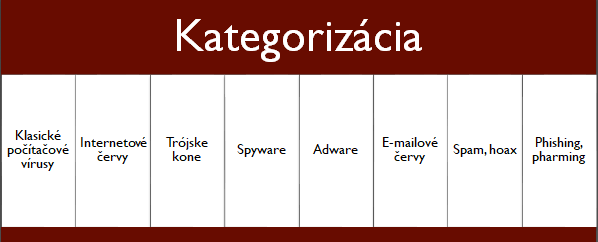
\includegraphics[scale=0.95]{malware_kategorizacia.png}
%\begin{center}
\begin{figure}[H]
Ďalšie dôležité informácie o~jednotlivých typoch malvéru nájdete \href{https://sk.wikipedia.org/wiki/Malware}{\textit{TU}}
%\end{center}
\end{figure}
\end{frame}

%-------------------------3rd page-------------------------
\begin{frame}
\frametitle{Vírusy}
\begin{itemize}
\item{Počítačový vírus je program, ktorý sa dokáže rozmnožovať pridávaním svojho kódu do iných programov
}
\item{Pre svoje rozširovanie teda podobne ako biologický vírus potrebuje hostiteľa – iný program
}
\item{Účinky nákazy počítača vírusom sú rozličné -- od vypísania "vtipných" textov až po zničenie dát uložených na diskoch
}
\item{Špeciálnym druhom vírusov sú Makro vírusy, rozšírené najmä v~prostredí kancelárskeho balíka MS Office(Word, Excel, PowerPoint, Outlook…)
}
\item{Pre viac informácii o~vírusoch kliknite na odkaz  \href{https://sk.wikipedia.org/wiki/Malware}{\textit{TU}}
}
\end{itemize}
\end{frame}

%-------------------------4th page-------------------------
\begin{frame}
\frametitle{Trójske kone}
\begin{itemize}
\item{Trójsky kôň (pomenovanie podľa trójskeho koňa z~Homérovho diela Illias) je škodlivý kód pribalený k~zdanlivo neškodnému softvéru
}
\item{Je to počítačový program, ktorý vykonáva deštruktívnu činnosť, pričom sa skrýva za „užitočnú“činnosť 
}
\item{Môžu mať najrôznejšie účinky (Padnutie systému, úprava alebo vymazanie dát, formátovanie diskov- strata celého obsahu, šírenie malvéru po sieti a~i.)
}
\vfill
\hspace{50mm}
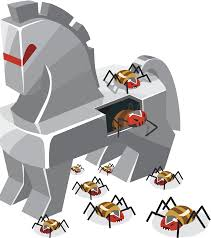
\includegraphics[scale=0.35]{malware_trojan_horse.jpg}
\end{itemize}
\end{frame}

%-------------------------5th page-------------------------
\begin{frame}
\frametitle{Spyware}
\begin{itemize}
\item{Škodlivé programy, ktoré sú vytvorené s~cieľom neeticky sa obohatiť
}
\item{Tieto programy zisťujú informácie o počítači a~jeho používateľovi a~bez súhlasu odosielajú cudzej osobe (napr. získanie zoznamu emailových adries, zoznam najčastejšie navštevovaných stránok, atď. )
}
\item{Najnebezpečnejším druhom spywaru sú tzv. keyloggery, ktoré zaznamenávajú všetky stlačené klávesy (získavajú prístupové heslá do počítačového systému, čísla kreditných kariet, registračné kľúče k~programom a~ďalšie informácie)
}
\item{Spywarom sú tiež niektoré programy vydávajúce sa za programy na odstraňovanie Spywaru ako napríklad Malware Wipe, Pest Trap, SpyAxe, AntiVirus Gold, SpywareStrike, SpyFalcon, SpyTrooper a~mnohé ďalšie
}
\end{itemize}
\end{frame}

%-------------------------6th page-------------------------
\begin{frame}
\frametitle{Boj proti malwaru}
\begin{itemize}
\item{Najlepšou liečbou je prevencia}
\item{Odporúčania sú tieto:}
\begin{itemize}
\item{Zálohujte všetky svoje údaje na úložné disky.}
\item{Používajte menej rozšírený operačný systém, prehliadač a~poštového klienta.}
\item{Zabezpečte svoj počítač proti neoprávnenému vniknutiu}
\item{Nenavštevujte nebezpečné stránky a nesťahujte programy na sťahovanie hudby, filmov a programov}
\item{Nezverejňujte svoju emailovú adresu}
\item{Neotvárajte neznáme prílohy}
\item{Chráňte svoj počítač aktuálnym antivírovým systémom}
\item{Chráňte svoj počítač proti špionážnym programom}
\item{Vypnite automatické spúšťanie programu po vložení média (CD, DVD, USB DISK)}
\end{itemize}
\end{itemize}
\end{frame}
%-------------------------7th page-------------------------
\begin{frame}
\frametitle{Použité zdroje}
\begin{itemize}
\item{\href{https://sk.wikipedia.org/wiki/Malware}{https://sk.wikipedia.org/wiki/Malware}}
\item{\href{https://www.avast.com/cs-cz/c-malware}https://www.avast.com/cs-cz/c-malware}
\end{itemize}
\end{frame}
\end{document}
